% !TeX program = xelatex
% 目录和交叉引用至少需要连续编译两次；推荐在提交包根目录运行“编译报告.ps1”。
\documentclass[UTF8,a4paper,12pt]{ctexart}

\usepackage[margin=2.5cm]{geometry}
\usepackage{amsmath,amssymb,bm}
\usepackage{booktabs,array}
\usepackage{graphicx,float,caption}
\usepackage{xcolor,hyperref}
\usepackage{siunitx}
\usepackage{fancyhdr}

\DeclareSIUnit\pixel{px}
\sisetup{detect-all}
\captionsetup{font=small,labelfont=bf}
\hypersetup{colorlinks=true,linkcolor=blue!55!black,urlcolor=blue!55!black,
  pdftitle={张氏平面相机标定实验报告}}

\newcommand{\StudentName}{贾宇航}
\newcommand{\StudentID}{26125201}
\newcommand{\CourseName}{机器视觉}

% 页眉：左侧为课程名称，中间为当前章节，右侧为页码。
\setlength{\headheight}{15pt}
\pagestyle{fancy}
\fancyhf{}
\fancyhead[L]{\CourseName}
\fancyhead[C]{\nouppercase{\leftmark}}
\fancyhead[R]{\thepage}
\renewcommand{\headrulewidth}{0.4pt}
\renewcommand{\footrulewidth}{0pt}
\renewcommand{\sectionmark}[1]{\markboth{#1}{}}
\fancypagestyle{plain}{
  \fancyhf{}
  \fancyhead[L]{\CourseName}
  \fancyhead[C]{\nouppercase{\leftmark}}
  \fancyhead[R]{\thepage}
  \renewcommand{\headrulewidth}{0.4pt}
  \renewcommand{\footrulewidth}{0pt}
}

\title{张氏平面相机标定实验报告}
\author{课程：\CourseName\qquad \StudentName\quad 学号：\StudentID}
\date{\today}

\begin{document}
\maketitle
\thispagestyle{empty}

\begin{abstract}
本实验利用多幅平面棋盘格图像完成张氏相机标定。程序在 $720\times576$ 像素图像中检测 $6\times4$ 个棋盘内角点，经亚像素优化后，从 19 个编号组中选取 38 个视图进行标定。实验估计了相机内参、OpenCV 五参数畸变模型及各视图外参，并用总体与逐图重投影误差评价结果。最终总体重投影 RMS 为 \SI{1.853}{\pixel}。结果表明镜头存在明显桶形畸变，去畸变后棋盘和背景线条得到显著校正；边缘视图的误差仍较大，说明强广角成像、视角倾斜及模型近似是主要误差来源。

\textbf{关键词：}张氏标定；棋盘格；相机内参；镜头畸变；重投影误差
\end{abstract}

\clearpage
\tableofcontents
\clearpage

\section{实验目的}

\begin{enumerate}
  \item 掌握由多幅平面棋盘格图像估计相机参数的张氏标定方法；
  \item 提取亚像素棋盘角点，估计内参、畸变参数和每幅图像的外参；
  \item 通过重投影误差和去畸变图像分析标定精度及主要误差来源。
\end{enumerate}

\section{数据与坐标约定}

数据根目录包含 23 个编号子目录，共 146 幅图像。主体数据为 $720\times576$ 像素、$6\times4$ 个内角点的棋盘格；部分目录包含其他分辨率或不同标定物。为保证所有视图共享同一内参模型，本实验只使用编号目录中分辨率为 $720\times576$ 的图像。在该分辨率下共有 126 幅图像成功检测到完整棋盘。

目录中的 \texttt{calibration\_images.zip} 是另一套 $1920\times1080$ 像素、$7\times7$ 个内角点的棋盘数据。它与编号目录的分辨率、棋盘规格和成像内容不同，不能混入同一内参模型，因此未纳入本实验。

程序将每个编号组的候选图像按文件名字典序排列，再等间隔抽取最多 2 幅，最终使用 19 组共 38 幅图像。这 38 幅原始图像已按编号组保存在本文件夹的 \texttt{棋盘格标定图片} 子目录中。图像坐标原点位于左上角，$u$ 轴向右、$v$ 轴向下；棋盘位于世界平面 $Z=0$。由于没有提供方格实际边长，令相邻内角点间距为 1，故平移向量以“一个方格边长”为单位，内参、畸变和旋转不受该尺度选择影响。

\section{张氏标定原理}

\subsection{平面单应性}

针孔相机模型为
\begin{equation}
  s\bm x=K[R\mid\bm t]\bm X,
  \qquad
  K=\begin{bmatrix}
  f_x&s_k&u_0\\
  0&f_y&v_0\\
  0&0&1
  \end{bmatrix}.
\end{equation}
棋盘位于 $Z=0$ 时，有
\begin{equation}
  \lambda\begin{bmatrix}u\\v\\1\end{bmatrix}
  =K[\bm r_1\ \bm r_2\ \bm t]
  \begin{bmatrix}X\\Y\\1\end{bmatrix}
  =H\begin{bmatrix}X\\Y\\1\end{bmatrix},
\end{equation}
其中 $H=[\bm h_1\ \bm h_2\ \bm h_3]$ 是棋盘平面到图像平面的单应矩阵。

\subsection{内参与外参求解}

定义
\begin{equation}
  B=K^{-T}K^{-1}.
\end{equation}
由旋转矩阵前两列正交且等模，可得
\begin{equation}
  \bm h_1^TB\bm h_2=0,
  \qquad
  \bm h_1^TB\bm h_1-\bm h_2^TB\bm h_2=0.
\end{equation}
每幅图像提供两个独立约束，多视图联合求解 $B$ 后即可恢复内参矩阵 $K$。本实验使用的 OpenCV 实现固定像素轴倾斜 $s_k=0$。

求得 $K$ 后，每幅图像的外参初值为
\begin{align}
  \bm r_1&=\lambda K^{-1}\bm h_1,&
  \bm r_2&=\lambda K^{-1}\bm h_2,\\
  \bm r_3&=\bm r_1\times\bm r_2,&
  \bm t&=\lambda K^{-1}\bm h_3,
\end{align}
其中 $\lambda=1/\lVert K^{-1}\bm h_1\rVert$。最终使用 Levenberg--Marquardt 方法联合优化内参、外参和畸变参数，使全部角点的重投影误差最小。

\subsection{畸变模型与评价指标}

本实验采用 OpenCV 五参数模型 $(k_1,k_2,p_1,p_2,k_3)$。令 $r^2=x^2+y^2$，归一化坐标的畸变关系为
\begin{align}
  x_d={}&x(1+k_1r^2+k_2r^4+k_3r^6)+2p_1xy+p_2(r^2+2x^2),\\
  y_d={}&y(1+k_1r^2+k_2r^4+k_3r^6)+p_1(r^2+2y^2)+2p_2xy.
\end{align}

设第 $i$ 幅图像的第 $j$ 个观测角点和重投影点分别为 $\bm q_{ij}$、$\hat{\bm q}_{ij}$，逐图误差为
\begin{equation}
  e_i=\sqrt{\frac{1}{N_i}\sum_{j=1}^{N_i}
  \lVert\bm q_{ij}-\hat{\bm q}_{ij}\rVert_2^2}.
\end{equation}
总体 RMS 对所有视图中的全部角点统一统计。

\section{实验步骤}

\begin{enumerate}
  \item 筛选 $720\times576$ 像素图像；
  \item 使用 \texttt{findChessboardCorners} 检测 $6\times4$ 个内角点；
  \item 使用 \texttt{cornerSubPix} 进行亚像素优化；
  \item 以单位方格坐标生成棋盘平面的三维点；
  \item 使用 \texttt{cv2.calibrateCamera} 估计内参、畸变及各视图外参；
  \item 根据逐图 RMSE 的中位数和 MAD 检查异常视图；
  \item 输出角点图、参数文件、逐图误差表和去畸变对比图。
\end{enumerate}

\section{实验结果}

\subsection{棋盘格标定图片}

图~\ref{fig:corners} 展示了误差最低和最高的若干视图。检测到的角点顺序和棋盘结构正确；误差较大的视图通常倾角更大或更靠近图像边缘。

\begin{figure}[H]
  \centering
  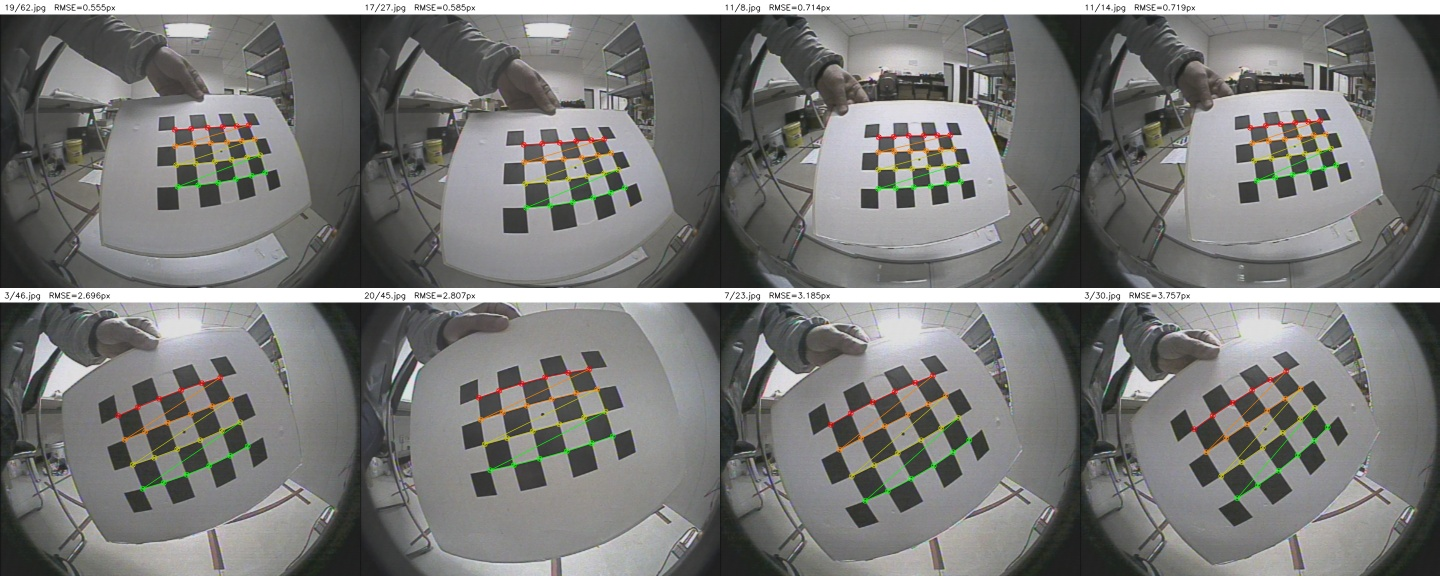
\includegraphics[width=\textwidth]{棋盘格角点检测.jpg}
  \caption{棋盘格亚像素角点检测结果}
  \label{fig:corners}
\end{figure}

\subsection{标定参数}

38 个视图均通过异常值检查。得到相机内参矩阵
\begin{equation}
  K=\begin{bmatrix}
  234.8668&0&330.2824\\
  0&258.3118&289.7628\\
  0&0&1
  \end{bmatrix}.
\end{equation}
五个畸变系数为
\begin{equation}
  (k_1,k_2,p_1,p_2,k_3)=
  (-0.315124,\ 0.122474,\ -0.004850,\ 0.007230,\ -0.023786).
\end{equation}

\begin{table}[H]
  \centering
  \caption{重投影误差统计}
  \begin{tabular}{lr}
    \toprule
    指标 & 数值/像素\\
    \midrule
    总体重投影 RMS & 1.853\\
    逐图 RMSE 均值 & 1.672\\
    逐图 RMSE 中位数 & 1.621\\
    最小逐图 RMSE & 0.555\\
    最大逐图 RMSE & 3.757\\
    \bottomrule
  \end{tabular}
\end{table}

\subsection{去畸变结果}

\begin{figure}[H]
  \centering
  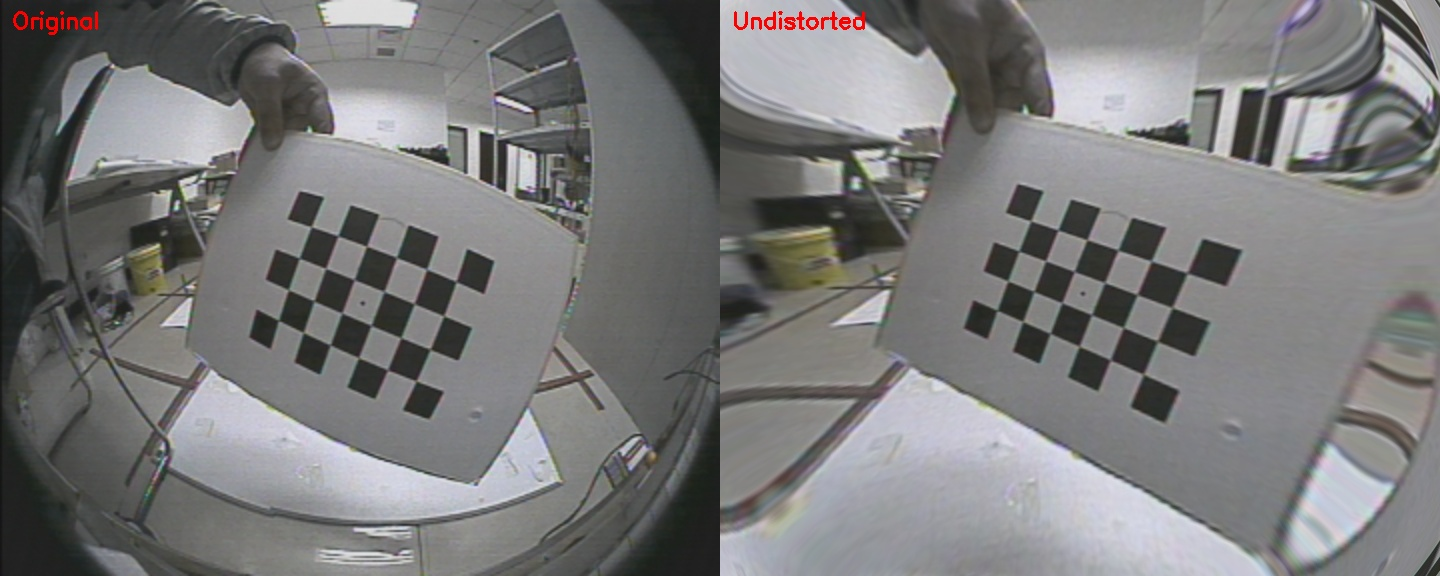
\includegraphics[width=\textwidth]{畸变校正对比.jpg}
  \caption{原始图像与去畸变结果对比}
  \label{fig:undistort}
\end{figure}

图~\ref{fig:undistort} 表明，校正后棋盘边缘和背景直线明显变直，同时图像边缘出现较强拉伸，这是广角图像几何展开时的正常现象。

\section{结果分析}

\begin{itemize}
  \item $k_1<0$ 表明存在明显桶形畸变；$k_2$ 与 $k_3$ 用于补偿高阶径向变化。
  \item 主点 $(330.28,289.76)$ 与图像中心 $(360,288)$ 的纵向位置接近，横向相差约 \SI{29.7}{\pixel}。该偏移可能来自真实光轴偏置、裁剪或强畸变与主点参数的耦合。
  \item $f_x/f_y\approx0.909$，未严格满足方形像素假设。可能原因包括成像或缩放过程，也可能是普通针孔加五参数模型对强广角成像的近似误差。
  \item 总体 RMS 为 \SI{1.853}{\pixel}，但逐图最大误差达到 \SI{3.757}{\pixel}，说明边缘、大倾角视图仍存在系统误差。
  \item 当前误差由参与标定的角点计算，只能表示拟合程度。若用于高精度测量，应保留独立验证图像，并检查残差是否随半径或图像位置呈系统变化。
  \item 数据未提供真实方格边长，因此外参平移只具有相对尺度，不能直接解释为毫米或厘米。
\end{itemize}

\section{复现说明}

本文件夹包含张氏标定代码 \texttt{calibrate\_zhang.py}、实际使用的 38 幅原始棋盘图、参数结果、逐图误差表和实验图片。进入本文件夹后可直接使用包内数据复现，\texttt{--output .} 表示把结果写入当前文件夹：
\begin{verbatim}
python -m pip install -r ..\requirements.txt
python calibrate_zhang.py --data .\棋盘格标定图片 --output .
\end{verbatim}

\section{结论}

本实验利用 38 幅棋盘格图像完成张氏标定，得到相机内参、五参数畸变和各视图外参，总体重投影 RMS 为 \SI{1.853}{\pixel}。结果正确反映了镜头的桶形畸变，去畸变图像的直线结构得到明显改善。边缘视图误差较大，后续可通过增加图像边缘和不同倾角的高质量视图、设置独立验证集以及比较其他畸变模型进一步提高可靠性。

\begin{thebibliography}{9}
\bibitem{zhang2000} Z. Zhang, ``A Flexible New Technique for Camera Calibration,'' \emph{IEEE TPAMI}, vol. 22, no. 11, pp. 1330--1334, 2000.
\bibitem{opencv} OpenCV Documentation, ``Camera Calibration and 3D Reconstruction,'' \url{https://docs.opencv.org/4.x/d9/d0c/group__calib3d.html}.
\end{thebibliography}

\end{document}
